% TikZ Figure: Parameter Sensitivity Heatmap (Fixed Legend)
% Standalone LaTeX file for generating PDF figure
\documentclass[tikz,border=5pt]{standalone}
\usepackage{pgfplots}
\pgfplotsset{compat=1.18}
\usepgfplotslibrary{colorbrewer}
\usepackage{amsmath}

\begin{document}
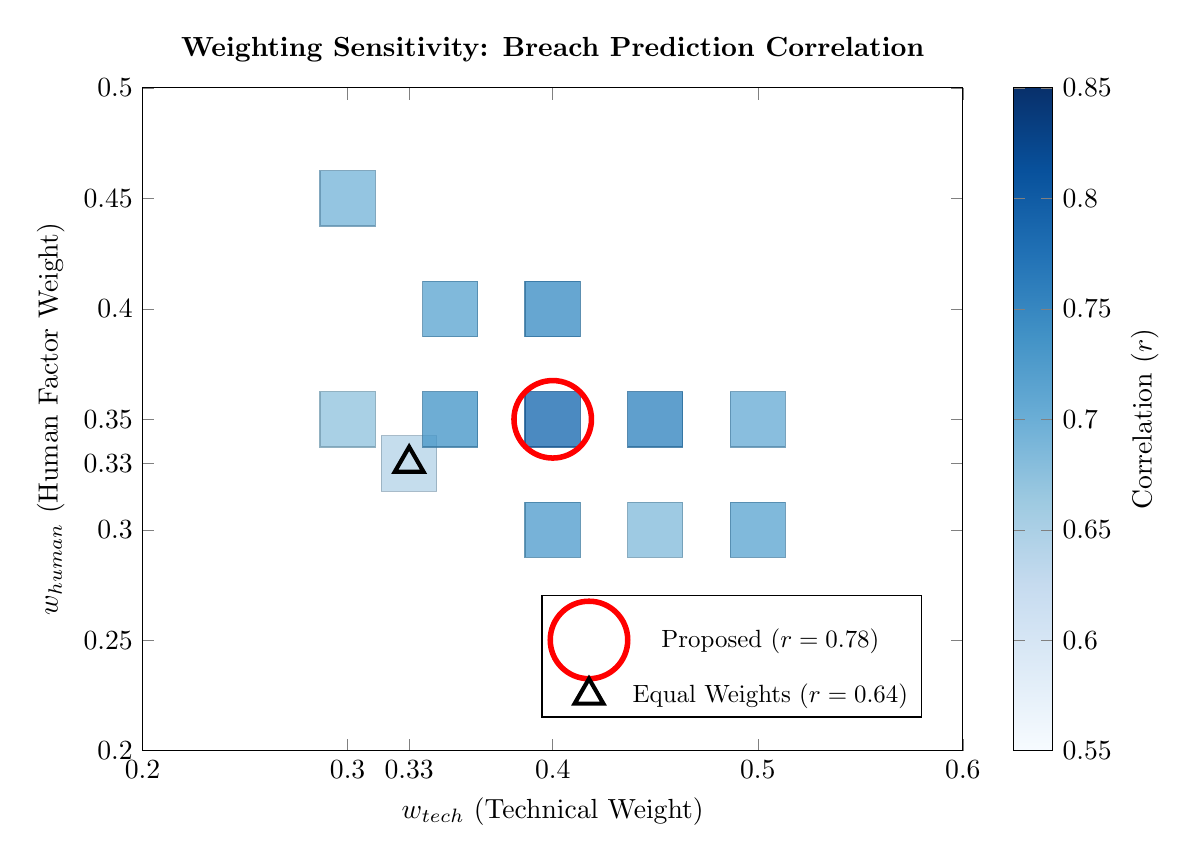
\begin{tikzpicture}
\begin{axis}[
    title={\textbf{Weighting Sensitivity: Breach Prediction Correlation}},
    xlabel={$w_{tech}$ (Technical Weight)},
    ylabel={$w_{human}$ (Human Factor Weight)},
    xmin=0.2, xmax=0.6,
    ymin=0.2, ymax=0.5,
    xtick={0.2,0.3,0.33,0.4,0.5,0.6},
    xticklabels={0.2,0.3,0.33,0.4,0.5,0.6},
    ytick={0.2,0.25,0.3,0.33,0.35,0.4,0.45,0.5},
    yticklabels={0.2,0.25,0.3,0.33,0.35,0.4,0.45,0.5},
    colorbar,
    colorbar style={
        ylabel={Correlation ($r$)},
    },
    colormap/Blues,
    point meta min=0.55,
    point meta max=0.85,
    width=12cm,
    height=10cm,
    legend style={at={(0.95,0.05)},anchor=south east,nodes={scale=0.9, transform shape}},
]

% 1. All Data Points (Heatmap Layer)
% Added 'forget plot' so this does NOT mess up the legend
\addplot[
    scatter,
    only marks,
    scatter src=explicit,
    mark=square*,
    mark size=10pt,
    opacity=0.8,
    forget plot
] coordinates {
    (0.33, 0.33) [0.64]
    (0.50, 0.30) [0.71]
    (0.30, 0.45) [0.69]
    (0.40, 0.35) [0.78]
    (0.45, 0.35) [0.75]
    (0.35, 0.35) [0.73]
    (0.40, 0.30) [0.72]
    (0.40, 0.40) [0.74]
    (0.50, 0.35) [0.70]
    (0.35, 0.40) [0.71]
    (0.45, 0.30) [0.68]
    (0.30, 0.35) [0.67]
};

% 2. Highlight: Proposed Model
\addplot[
    only marks,
    mark=o,
    mark size=14pt,
    line width=2pt,
    color=red,
] coordinates {(0.40, 0.35)};
\addlegendentry{Proposed ($r=0.78$)}

% 3. Highlight: Equal Weights
\addplot[
    only marks,
    mark=triangle,
    mark size=6pt,
    line width=1.5pt,
    color=black,
] coordinates {(0.33, 0.33)};
\addlegendentry{Equal Weights ($r=0.64$)}

\end{axis}
\end{tikzpicture}
\end{document}
